\documentclass[a4paper]{article}

% Umlaute
\usepackage[T1]{fontenc}
% Wir wollen auch Umlaute schreiben
\usepackage[utf8]{inputenc}

\usepackage[ngerman]{babel}

\usepackage{graphicx}

% Unsere Makros
\newcommand*{\ddsg}[2][Donau]{#1dampfschifffahrts#2}
\newcommand*{\dx}[1][x]{\;\mathrm{d}#1}
\newcommand*{\N}[1][]{\mathbb{N}^{#1}}

\title{Blöder Titel}
\author{ich}
\date{\today}

% Mathe-Pakete
\usepackage{amsmath}
\usepackage{amsfonts}
\usepackage{amssymb}
\usepackage{amsthm}

% Für Theorem und seine Freunde
\usepackage{thmtools}

\declaretheorem[
name=Theorem,
style=theorem,
numberwithin=section
]{thm}
\declaretheorem[
name=Lemma,
style=theorem,
sibling=thm,
]{lem}
\declaretheorem[
name=Proposition,
style=theorem,
sibling=thm,
]{prop}

\declaretheorem[
name=Definition,
style=definition,
numbered=no,
]{defin}

\declaretheorem[
name=Bemerkung,
style=remark,
numbered=no
]{rem}

% Bibliographie
\usepackage[style=numeric,
            backend=biber,
            doi=false,isbn=false,url=false,
            ]{biblatex}
\addbibresource{./content/references.bib}

% Ich komme immer zum Schluss!
\usepackage{hyperref}

\begin{document}
\part{16.10.2015}
\section{Umlaute und aktuelle deutsche Rechtschreibung}
Fix Schwyz quäkt Jürgen blöd vom Paß.
The quick brown fox jumps over the lazy dog.

Binde immer \verb+\usepackage[T1]{fontenc}+, \verb+\usepackage[utf8]{inputenc}+ und \verb+\usepackage[ngerman]{babel}+ ein!

\section{Titel}
\maketitle % Titel

Siehe \verb+\author, \title+ und \verb+\date+

\section{Überschriften}

\section{Eine Überschrift}
\subsection{Eine Unterüberschrift}
\subsubsection{Eine Unterunterüberschrift}
\paragraph{Test}
\subparagraph{Sub-Test}

\tableofcontents

\section{Ein kurzer Abschnitt} \label{sec:Ein kurzer Abschnitt}
Auch gibt es niemanden, der den Schmerz an sich liebt, sucht oder wünscht, nur, weil er Schmerz ist, es sei denn, es kommt zu zufälligen Umständen, in denen Mühen und Schmerz ihm große Freude bereiten können. Um ein triviales Beispiel zu nehmen, wer von uns unterzieht sich je anstrengender körperlicher Betätigung, außer um Vorteile daraus zu ziehen? Aber wer hat irgend ein Recht, einen Menschen zu tadeln, der die Entscheidung trifft, eine Freude zu genießen, die keine unangenehmen Folgen hat, oder einen, der Schmerz vermeidet, welcher keine daraus resultierende Freude nach sich zieht? Auch gibt es niemanden, der den Schmerz an sich liebt, sucht oder wünscht, nur, weil er Schmerz ist, es sei denn, es kommt zu zufälligen Umständen, in denen Mühen und Schmerz ihm große Freude bereiten können. Um ein triviales Beispiel zu nehmen, wer von uns unterzieht sich je anstrengender körperlicher Betätigung, außer um Vorteile daraus zu ziehen? Aber wer hat irgend ein Recht, einen Menschen zu tadeln, der die Entscheidung trifft, eine Freude zu genießen, die keine unangenehmen Folgen hat, oder einen, der Schmerz vermeidet, welcher keine daraus resultierende Freude nach sich zieht?Auch gibt es niemanden, der den Schmerz an sich liebt, sucht oder wünscht, nur, 


\section{Querverweise}
Wie wir in Abschnitt~\ref{sec:Ein kurzer Abschnitt} gesehen haben, gilt ...

\url{tim.benedikt.herbstrith@univie.ac.at}

\href{mailto:tim.benedikt.herbstrith@univie.ac.at}{Schreib mir ein Mail!}

Springe im Dokument mit \verb+\usepackage{hyperref}+ (muss immer an letzter Stelle stehen!).

\section{Textschnitte}
Ich bin \textbf{fett.} \textit{kursiv,} \textsl{slanted,} \texttt{Schreibmaschine,}
\textsc{Kapitälchen}

\emph{Fix Schwyz} quäkt Jürgen blöd vom Paß.
The quick brown fox jumps over the lazy dog.

\textit{Fix Schwyz} quäkt Jürgen blöd vom Paß.

\itshape
Ab hier alles kursiv: Testtext

Fix Schwyz quäkt Jürgen blöd vom Paß.
The quick brown fox jumps over the lazy dog.
\upshape

\section{Bilder}

Hier kommt ein Bild (siehe Abb.~\ref{im:Bibel})

\begin{figure}
\begin{center}
    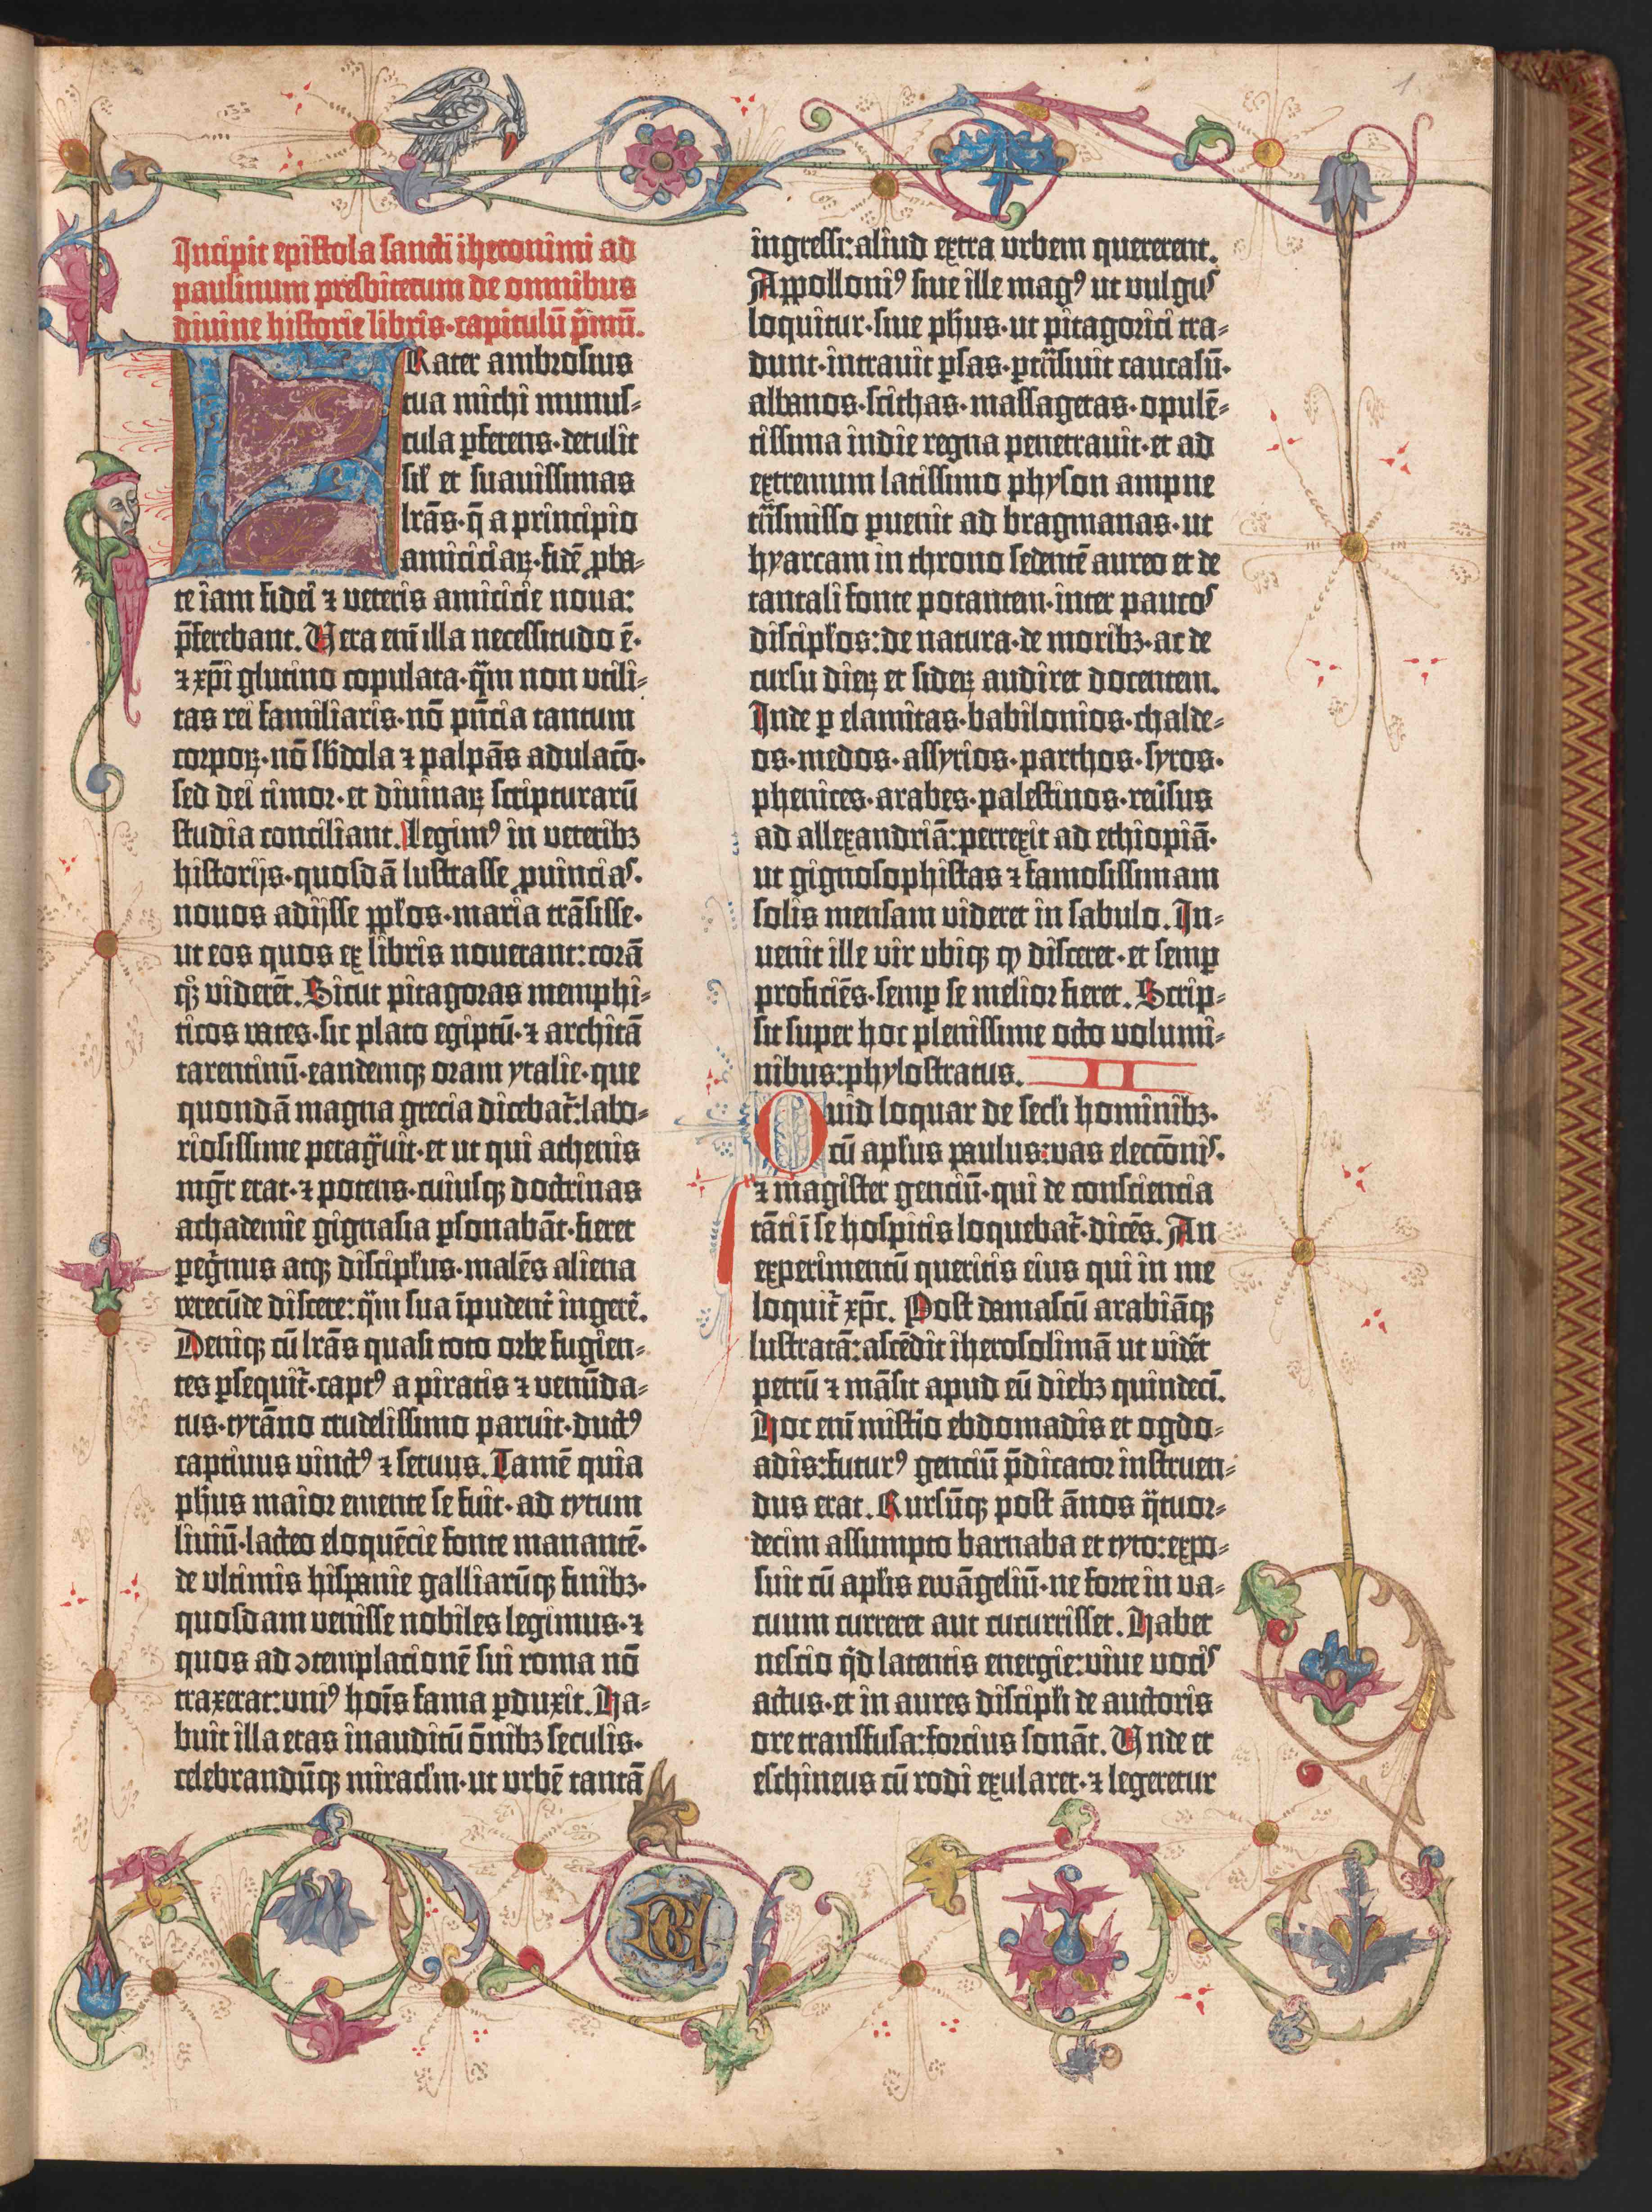
\includegraphics[width=0.5\textwidth]{./res/gutenberg.jpg}
\caption{Gutenberg Bibel}
\label{im:Bibel}
\end{center}
\end{figure}

Hier geht es weiter.
\listoffigures

Binde \verb+\usepackage{graphicx}+ ein.

\section{Tabellen}
Hier kommt Text.
\begin{table}[tbp]
\begin{center}
\begin{tabular}{|p{2cm}|c r|}
\hline
links    &    mitte    &    rechts\\
\hline
Zweile   &    Zwei     &    !\\
Donau\-dampf\-schiff\-fahrts\-ge\-sell\-schaft&&\\
\hline
\hline
\end{tabular}
\caption{Eine Tabelle}
\label{tab:Tabelle}
\end{center}
\end{table}
Und noch mehr Text, der auf die Tabelle verweist (siehe Tab.~\ref{tab:Tabelle}).
\listoftables

\newpage
\part{23.10.2015}

\section{Listen und Aufzählungen}

\begin{itemize}
\item Bullet 1
\item Bullet 2
\end{itemize}

\begin{enumerate}
\item Listeneintrag 1
\item Listeneintrag 2\label{item:List 1}
\end{enumerate}

Ich beziehe mich auf Eintrag~\ref{item:List 1}.

\begin{description}
\item[Felis silvestris catus] die Katze
\end{description}

Einkaufsliste
\begin{itemize}
\item Supermarkt
\begin{enumerate}
\item Zwiebel
\item[x] Äpfel
\item Milch
\end{enumerate}
\item Bauhaus
\begin{enumerate}
\item Hammer
\item Nägel
\end{enumerate}
\end{itemize}

\section{Externe Dokumente}

Ich bin ein Text, der nicht im Hauptdokument steht.


\section{Makros}

Geschwungene Klammern für Abstand
\ddsg{gesellschaft} + \ddsg[Inn]{-AG}skapitän

\section{Mathematik}
\subsection{Einfache Formeln}
Eine einfache Formel $2 a x=2$. Hier geht es weiter. \ddsg{} \ddsg{} \ddsg{} \ddsg{}  \ddsg{} \ddsg{} \ddsg{} \ddsg{} \ddsg{} \ddsg{} \ddsg{} \ddsg{} \ddsg{} \ddsg{} \ddsg{} \ddsg{} \ddsg{} \ddsg{} \ddsg{} \ddsg{}

Sei $a = 2$, dann ist $a$ eine Primzahl.\ddsg{} \ddsg{} \ddsg{} \ddsg{}  \ddsg{} \ddsg{} \ddsg{} \ddsg{} \ddsg{} \ddsg{} \ddsg{} \ddsg{} \ddsg{} \ddsg{} \ddsg{} \ddsg{} \ddsg{} \ddsg{} \ddsg{} \ddsg{}

So kann eine längere Gleichung aussehen
\[
4ac + 3a - b.
\]
Hier geht es weiter.

Wir können auch die quadratische Lösungsformel angeben:
\[
x_{1,2} = \frac{p}{2} \pm \sqrt{\frac{p^2}{4} - q}
\]

Die kummulierte Wahrscheinlichkeitsfunktion der Normalverteilung:
\[
\Phi(t) = \frac{1}{\sqrt{2\pi}\sigma} \int_{-\infty}^{t} e^{-\frac{(x-\mu)^2}{2 \sigma^2}} \dx
\]

\subsection{Klammern aller Formen und Größen}
Die kummulierte Wahrscheinlichkeitsfunktion der Normalverteilung:
\[
\Phi(t) = \frac{1}{\sqrt{2\pi}\sigma} \int_{-\infty}^{t} e^{-\frac{\left(\dfrac{x-\mu}{\sigma}\right)^2}{2}} \dx
\]

Eine Menge:
\[
M := \left\lbrace\frac{1}{x^2} \;\middle\vert\; x\in N \right\rbrace
\]

\[
M := \left\lbrace 2x \mid x\in N \right\rbrace
\]

\subsection{Textschnitte im \emph{Mathe}-Modus}
\[
\mathrm{f},\mathit{f}, \mathtt{f}, \mathfrak{ABC}, \mathcal{ABC}, \mathbb{F}
\]

\[
M := \left\lbrace 2x \mid x\in \N[*] \right\rbrace
\]

\[
A = 
\begin{pmatrix}
1 & 2\\
3 & 4\\
\end{pmatrix}
\]

\subsection{Nummerierung und mehrere Zeilen}

\begin{equation}
A = 
\begin{pmatrix}
1 & 2\\
3 & 4\\
\end{pmatrix}\label{eq:Eine Gleichung}
\end{equation}

\begin{align}
a &= b\nonumber\\
ab &= b^2\nonumber\\
a^2 - ab &= a^2 - b^2\\
(a-b)a &= (a-b)(a + b)\nonumber\\
a &= a+b\nonumber\\
0 &= b
\end{align}

Wie wir in Gleichung~\ref{eq:Eine Gleichung} gesehen haben, ...

Keine Zeilennummern
\begin{equation*}
A = 
\begin{pmatrix}
1 & 2\\
3 & 4\\
\end{pmatrix}\label{eq:Eine Gleichung}
\end{equation*}

\begin{align*}
a &= b\\
ab &= b^2\\
a^2 - ab &= a^2 - b^2\\
(a-b)a &= (a-b)(a + b)\\
a &= a+b\\
0 &= b
\end{align*}


\subsection{Theoreme}

\begin{thm}[Ein besonders schwieriges]
Ein Theorem
\end{thm}
\begin{lem}
Ein Lemma
\end{lem}
\begin{defin}
Eine Definition
\end{defin}

\begin{rem}
Ich bemerke, es wird schon spät.
\end{rem}

\begin{proof}
Ein Beweis
\end{proof}

\section{Bibliographie}

Ich mag die Bücher \cite[\S~5, Abs.~7]{kafka2015prozess} und \cite{AC02615918}. \textcite{kafka2015prozess} schreibt tolle Bücher.

\printbibliography

\end{document}






